\documentclass[tikz, border=10pt]{standalone}
\usepackage{pgfplots}
\usepackage{amsmath}
\usetikzlibrary{backgrounds}
\pgfplotsset{compat=1.18}

\begin{document}
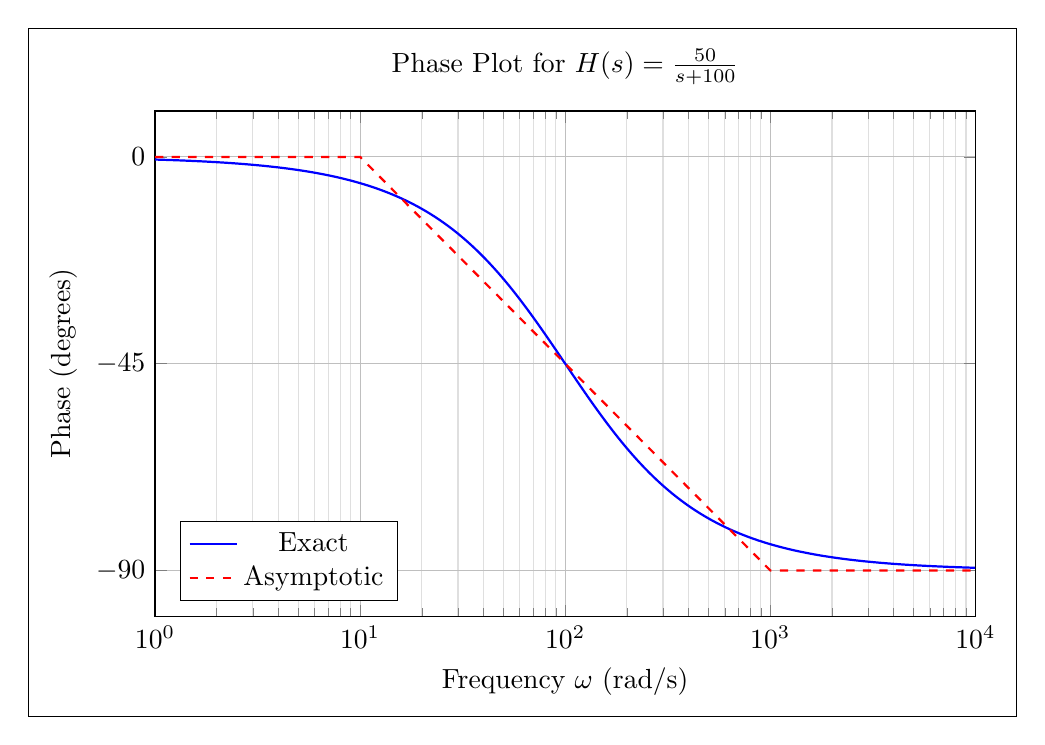
\begin{tikzpicture}[show background rectangle]
    \begin{semilogxaxis}[
        width=12cm, height=8cm,
        title={Phase Plot for $H(s) = \frac{50}{s+100}$},
        xlabel={Frequency $\omega$ (rad/s)},
        ylabel={Phase (degrees)},
        grid=both,
        xmin=1, xmax=10000,
        ymin=-100, ymax=10,
        minor grid style={gray!25},
        major grid style={gray!50},
        legend pos=south west,
        ytick={0, -45, -90},
    ]

    % Exact Phase: -atan(x/100)
    \addplot[blue, thick, domain=1:10000, samples=300] {-atan(x/100)};
    \addlegendentry{Exact}

    % Asymptotic Phase
    % Pole at 100: 0 until 10, then -45/dec until 1000, then -90
    \addplot[red, dashed, thick] coordinates {
        (1, 0) (10, 0) (1000, -90) (10000, -90)
    };
    \addlegendentry{Asymptotic}
    
    \end{semilogxaxis}
\end{tikzpicture}
\end{document}
